In this section the results based on the performed user tests and user evaluation are presented. There were 9 test users, whereof 2 were female and 7 were male. All of them were in their 20s and were studying at KTH.

\section{Effectiveness}

\subsection{Timescale} %Add standardavvikelse
Table \ref{avg_time} declares the average time in seconds it took for the users to complete each version of the game. The data shows that it takes 38\% more time to complete the speech version when compared to the text version.

\begin{table}[ht]
  \centering
  \begin{tabular}{ccc}
    \toprule
    Speech &   & Text\\
    \midrule
    445.22 &   & 310.22\\
    \bottomrule
  \end{tabular}
  \caption{Average time to complete the game}\label{avg_time}
\end{table}

\subsection{Commands} %Add standardavvikelse
Table \ref{avg_cmd} declares the average amount of commands used before completing the game. The data shows that it takes almost double the amount of commands (99.67\% more) to complete the speech version when compared to the text version. This can also be seen in figure \ref{ideal_cmd}, where the average amount of commands used in each version of the game are compared to the ideal number of commands for each version. The ideal takes in consideration a realistic first playthrough of the game, where the player does not ``magically know'' what items are in each room. Therefore, when entering a room, the command “search room” was used to get the list of items located in the room. No items in the rooms were checked, just taken and used, unless the puzzle involved looking at an item (e.g. searching the desk to find the key). In figure \ref{ideal_cmd} it is also shown that the ideal number of commands are pretty much the same for both versions of the game, making the difference in average number of commands even more significant.

\begin{table}[ht]
  \centering
  \begin{tabular}{ccc}
    \toprule
    Speech &   & Text\\
    \midrule
    64.33 &   & 31.22\\
    \bottomrule
  \end{tabular}
  \caption{Average number of commands used}\label{avg_cmd} % OMG LOOK HERE!!!
\end{table}

\begin{figure}[ht]
  \centering
  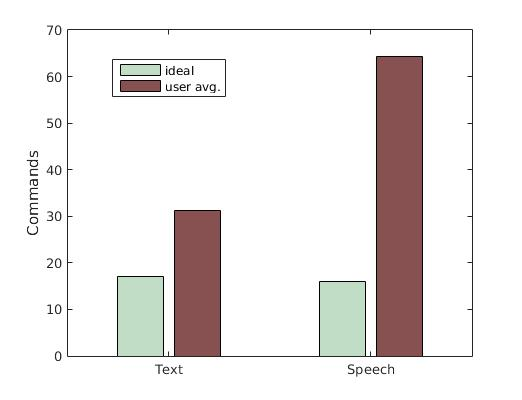
\includegraphics[width=0.8\textwidth]{images/ideal_cmd.jpg}
  \caption{Average amount of commands used compared to the ideal}\label{ideal_cmd}
\end{figure}

Figure \ref{time_cmd} shows the number of commands used over time. As you would expect, the speech version follows the logic of ``the longer time played the more commands used''. However, this is not the case for the text version, where the time played seems irrelevant to the amount of commands used.

\begin{figure}[ht]
  \centering
  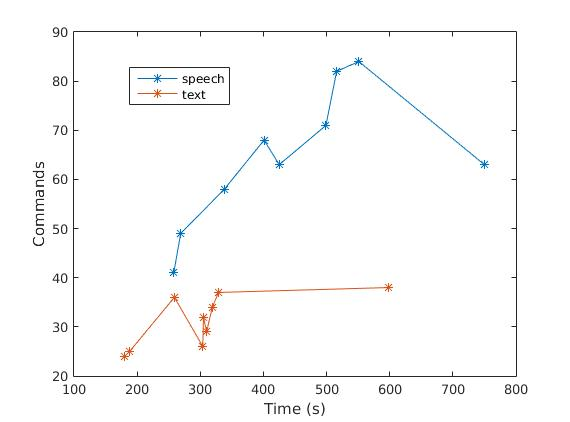
\includegraphics[width=0.8\textwidth]{images/time_cmd.jpg} %width=0.8\textwidth scales the image down to 80 percent of the text-width. Keeps the ratio.
  \caption{Number of commands used over time}\label{time_cmd}
\end{figure}

\section{Ease of Use}
\subsection{English Confidence} \label{sec:eng_con}
Each user rated their spoken and written English on a scale 1-5, where 1 equals ``not good'' and 5 equals ``fluent''. The users were divided into groups based on their estimated English level and the average amount of commands, time played and usability score were calculated for each group. The results are presented in figure \ref{eng_cmd}, figure \ref{eng_time} and figure \ref{eng_score}. The average time for users of English level 4 did not differ much between versions, although for the users of English level 3 and 5 a more significant difference is shown.
\newpage
\begin{figure}[ht]
  \centering
  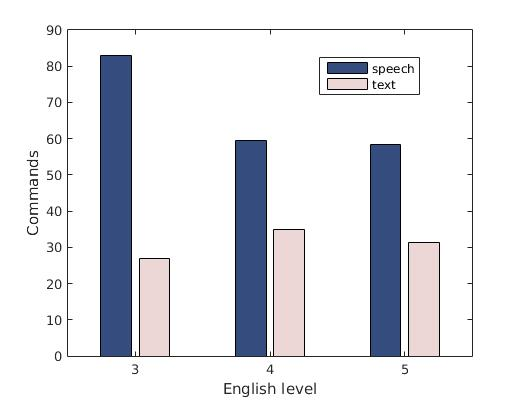
\includegraphics[width=0.8\textwidth]{images/english_cmd.jpg}
  \caption{Average amount of commands used per English level-group}\label{eng_cmd}
\end{figure}

\begin{figure}[H]
  \centering
  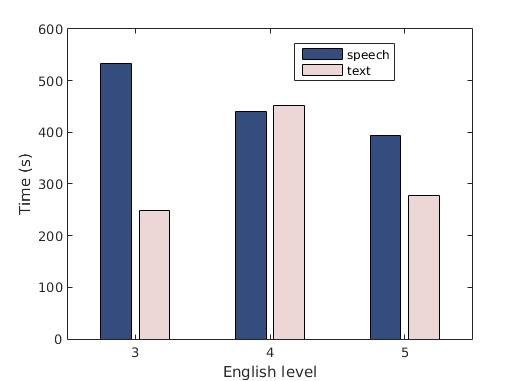
\includegraphics[width=0.8\textwidth]{images/english_time.jpg}
  \caption{Average time to complete the game per English level-group}\label{eng_time}
\end{figure}

\begin{figure}[H]
  \centering
  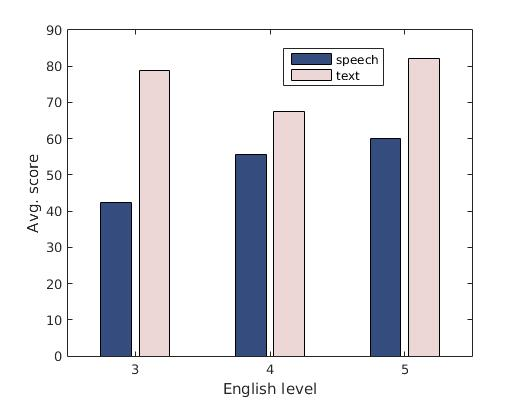
\includegraphics[width=0.8\textwidth]{images/english_score.jpg}
  \caption{Average score based on the SUS per English level-group}\label{eng_score}
\end{figure}

%\subsection{User Former Experience}
%\newpage
\section{Satisfaction (SUS)}
Figure \ref{fig:sus_table} shows the average score for each statement in the questionnaire described in section \ref{usability}. The scores have been converted according to formula \ref{eq:convert} in section \ref{sec:sus}. 

The average total usability score based on the SUS as calculated in formula \ref{eq:sum} for each version can be seen in table \ref{tot_score}. According to figure \ref{fig:susadj} speech can be considered OK and text considered good.

\begin{table}[ht]
  \centering
  \begin{tabular}{ccc}
    \toprule
    Speech &   & Text\\
    \midrule
    54.17 &   & 78.06\\
    \bottomrule
  \end{tabular}
  \caption{Average score based on the SUS}\label{tot_score}
\end{table}

\begin{figure}[ht]
  \centering
  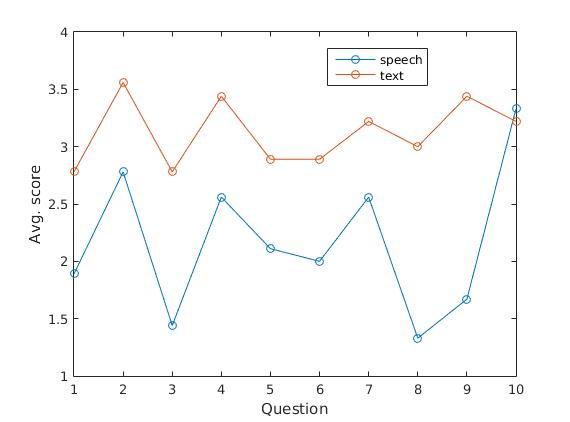
\includegraphics[width=0.8\textwidth]{images/sus.jpg}
  \caption{Average converted score for each statement}\label{fig:sus_table}
\end{figure}